\documentclass[10pt]{article}
\usepackage[spanish]{babel}
\usepackage[utf8]{inputenc}
\usepackage{geometry}
\newgeometry{top=2.3cm,bottom=3.5cm,right=2.5cm,left=2.5cm}
\usepackage{multicol}
\usepackage{graphicx}
\usepackage{url}
\usepackage{hyperref}
\usepackage{array}
\usepackage{tcolorbox}
\usepackage{xcolor} % define colores personalizados
\usepackage{listings}
\lstdefinestyle{ascii-tree}{
	literate={├}{|}1 {─}{--}1 {└}{+}1 
}
\lstset{basicstyle=\ttfamily,
	showstringspaces=false,
	commentstyle=\color{red},
	keywordstyle=\color{blue}
}

\usepackage{caption}

\newcolumntype{M}[1]{>{\centering\arraybackslash}m{#1}}

\newcommand{\itemCourse}{Estructura de Datos y Algoritmos}
\newcommand{\itemTheme}{Tries}
\newcommand{\itemPracticeNumber}{06}
\newcommand{\itemAcademic}{2023 - A}
\newcommand{\itemSemester}{III}
\newcommand{\itemDate}{19 Julio 2023}
\newcommand{\itemHour}{23:59 PM}

\newcommand{\itemEmail}{dninas@unsa.edu.pe}
\newcommand{\itemStudentA}{Coronado Peña Javier}
\newcommand{\itemStudentB}{Forocca Mamani Maxs Sebastian Joaquin}
\newcommand{\itemStudentC}{Diego Claudio Nina Suyo}

\newcommand{\itemTeacher}{Mg. Edith Giovanna Cano Mamani}

\newcommand{\itemUniversity}{Universidad Nacional de San Agustín de Arequipa}
\newcommand{\itemFaculty}{Facultad de Ingeniería de Producción y Servicios}
\newcommand{\itemDepartment}{Departamento Académico de Ingeniería de Sistemas e Informática}
\newcommand{\itemSchool}{Escuela Profesional de Ingeniería de Sistemas}
%%%%%%%%%%%%%%%%%%%%%%%%%%%%%%%%%%%%%%%%%%%%%%%%%%%%%%%%%%%%%%%%%%%%%%%%%%%%

\usepackage{tabularx}

\usepackage{fancyhdr}
\pagestyle{fancy}
\fancyhf{}

\renewcommand{\headrulewidth}{0pt}

\fancyhead[C]{
	\begin{tabularx}{\textwidth}{|M{3.8cm}|M{7.67cm}|M{3.8cm}|}
		\hline
		
\includegraphics[scale=0.45]{img/logo_episunsa.png} &\cellcolor{graya}{\textbf{\footnotesize\itemUniversity}\par\textbf{\footnotesize\itemFaculty}\par\textbf{\footnotesize\itemSchool}} & \vspace{0.16cm}
\includegraphics[scale=0.52]{img/logo_abet.png} \\
		\hline
		\multicolumn{3}{|c|}{\footnotesize \textbf{Formato:} Guía de Práctica de Laboratorio / Talleres / Centros de Simulación}\\
		\hline
		\cellcolor{graya}{\textbf{\footnotesize Aprobación: 2022/03/01}} & \textbf{\footnotesize Código: GUIA-PRLD-001} & \cellcolor{graya}{\textbf{\footnotesize Página: \thepage}} \\
		\hline
	\end{tabularx}}

\setlength{\headheight}{66pt} % Ajusta la altura del encabezado
\setlength{\headsep}{16pt} % Ajusta la separación entre el encabezado y el texto
\setlength{\footskip}{0pt} % Ajusta la separación entre el final del texto y el pie de página

% para el codigo fuente
\usepackage{listings}
\usepackage{color, colortbl}
\definecolor{dkgreen}{rgb}{0,0.6,0}
\definecolor{gray}{rgb}{0.5,0.5,0.5}
\definecolor{graya}{rgb}{0.97,0.97,0.97}
\definecolor{mauve}{rgb}{0.58,0,0.82}
\definecolor{codebackground}{rgb}{0.95, 0.95, 0.92}
\definecolor{tablebackground}{rgb}{0.8, 0, 0}

\lstset{frame=tb,
	language=bash,
	aboveskip=3mm,
	belowskip=3mm,
	showstringspaces=false,
	columns=flexible,
	basicstyle={\small\ttfamily},
	numbers=none,
	numberstyle=\tiny\color{gray},
	keywordstyle=\color{blue},
	commentstyle=\color{dkgreen},
	stringstyle=\color{mauve},
	breaklines=true,
	breakatwhitespace=true,
	tabsize=3,
	backgroundcolor= \color{codebackground},
}
\usepackage{lipsum}

\begin{document}
	
	\vspace*{0cm}	
	\begin{center}	
		\fontsize{17}{17} \Large{\textbf{INFORME DE LABORATORIO}}
	\end{center}
	%\centerline{\textbf{\Large Tema: \itemTheme}}
	%\vspace*{0.5cm}	
 
	\begin{table}[h!]
		\renewcommand{\arraystretch}{1.7}
  \footnotesize
		\begin{tabular}{|m{2.4cm}|m{2.1cm}|m{2.4cm}|m{2cm}|m{2.64cm}|m{2.42cm}|}
			\hline 
			\rowcolor{tablebackground}
			\multicolumn{6}{|c|}{\textbf{\large\color{white} INFORMACION BASICA}}\\ \hline
			%\multicolumn{6}{|c|}{\textsc{\Large\color{white} Información Básica}}\\
			{\cellcolor{graya}{ASIGNATURA:}} & \multicolumn{5}{l|}{\itemCourse}\\ \hline 
			\cellcolor{graya}{TITULO DE LA PRACTICA:} & \multicolumn{5}{l|}{\itemTheme}\\ \hline 
			\cellcolor{graya}{NUMERO DE LA PRACTICA:} & \itemPracticeNumber & \cellcolor{graya}{AÑO LECTIVO:} & \itemAcademic & \cellcolor{graya}{N° SEMESTRE:} & \itemSemester\\ \hline 
			\cellcolor{graya}{FECHA DE \par PRESENTACION:} & \itemDate & \cellcolor{graya}{HORA DE \par PRESENTACION:} & \multicolumn{3}{l|}{\itemHour} \\ \hline 
			\multicolumn{4}{|l|}{\begin{minipage}{8cm}
					\vspace{0.5em} % Espaciado ajustable según necesidad
					INTEGRANTE (s):
					%\vspace{-0.3cm}
					\begin{itemize}
						\setlength{\itemsep}{0pt}
						\setlength{\parskip}{0pt}
						\setlength{\parsep}{0pt}
						\item \itemStudentA
						\item \itemStudentB
						\item \itemStudentC
					\end{itemize}
					\vspace{0em} % Espaciado ajustable según necesidad
			\end{minipage}} & \cellcolor{graya}{NOTA:} & \\ \hline 
			\multicolumn{6}{|l|}{\begin{minipage}{8cm}
					\vspace{0.5em} % Espaciado ajustable según necesidad
					DOCENTE (s):
					%\vspace{-0.3cm}
					\begin{itemize}
						\setlength{\itemsep}{0pt}
						\setlength{\parskip}{0pt}
						\setlength{\parsep}{0pt}
						\item \itemTeacher
					\end{itemize}
					\vspace{0em} % Espaciado ajustable según necesidad
			\end{minipage}}\\ \hline 	
		\end{tabular}
	\end{table}
	\normalsize

 \section{Tarea}
\begin{itemize}
    \item Elabore un informe paso a paso de la implementación una Trie para insertar, buscar y reemplazar palabras en un texto.
    \item Utilice interfaces gráficas de usuario para su implementación.
    \item Utilice todas las recomendaciones dadas por el docente.
    \item Utilice la siguiente GUI como referencia:
    \begin{figure}[h!]
        \begin{center}
            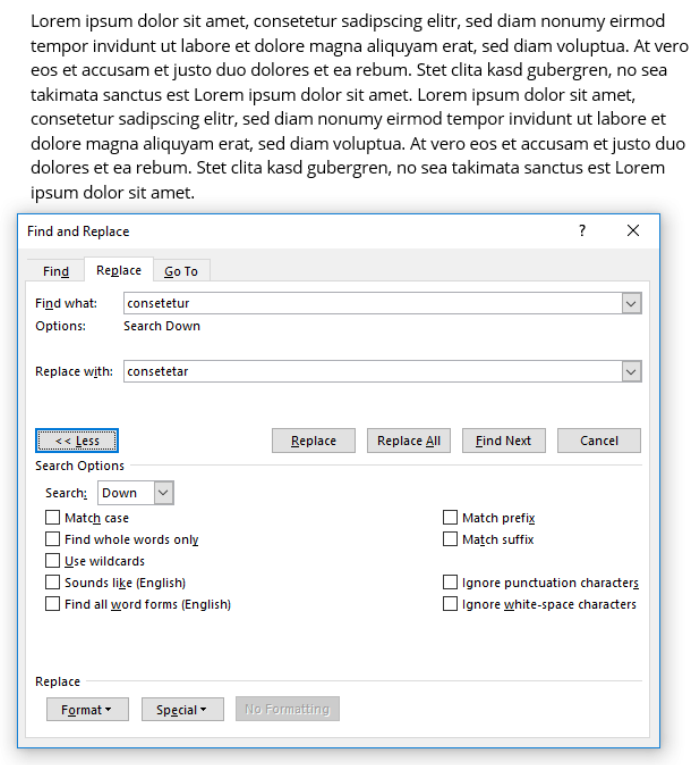
\includegraphics[scale=0.28]{img/GUI.png}
        \end{center}
    \end{figure}
\end{itemize}
\section{URL de Repositorio Github}
\begin{itemize}
    \item URL del Repositorio GitHub para clonar o recuperar.
    \item \url{https://github.com/DiegoNiS/Laboratorio-EDA-Colab.git}
\end{itemize}


% \section{Ejecuciones}


%\clearpage
\section{Pregunta}
\textbf{Explique. ¿Cómo se utiliza esta estructura de datos para almacenar prefijos?.}\\



\section{Pregunta}
\textbf{Explique. ¿Cómo se utiliza esta estructura de datos para almacenar prefijos?.}\\



\end{document}